\documentclass[11pt,a4paper]{memoir}

\usepackage{graphicx}
\usepackage{geometry}
\usepackage{float}
\usepackage{hyperref}
\usepackage[table]{xcolor}
\usepackage[backend=biber, style=numeric]{biblatex}

\addbibresource{bibliography.bib}

\hypersetup{
	colorlinks=true,
	linkcolor=black,
	urlcolor=blue,
	citecolor=black
}

\graphicspath{{figures/}}

\setsecnumdepth{subsection}

\renewcommand*{\maketitle}%
{
	\newgeometry{left=2cm,right=2cm,top=3cm,bottom=3.5cm}

	\begin{center}
		\begingroup
		{\Huge\textbf{POLITECNICO DI TORINO}}\\[\baselineskip]
		\rule{\textwidth}{2pt}\par
		\vspace*{1em}
		{\LARGE\textbf{Master's Degree in Computer Engineering}}\\[\baselineskip]
		\vspace*{1em}
		{\Large\textbf{Master's Degree Thesis}}\\
		\vspace*{2cm}
		{\huge\textbf{Acceleration by Separate-Process Cache for
		Memory-Intensive Algorithms on FPGA via High-Level Synthesis}}\\
		\vspace*{1cm}
		
\includegraphics[width=.3\textwidth]{figures/polito-logo}
	\end{center}
	\vfill
	\begin{minipage}{0.4\textwidth}
		\begin{flushleft}
			{\Large
				\textbf{Supervisor}\\
				Prof. Luciano Lavagno
			}
		\end{flushleft}
	\end{minipage}
	\begin{minipage}{0.4\textwidth}
		\begin{flushright} 
			{\Large
				\textbf{Candidate}\\
				Giovanni Brignone\\
				ID: 274148
			}
		\end{flushright}
	\end{minipage}  
	\vspace*{2cm}
	\begin{center}
		{\Large\textbf{Academic year 2020-2021}}
	\end{center}
	\endgroup

	\restoregeometry 
}

\begin{document}
\pagestyle{empty}
\maketitle

\frontmatter
\chapter*{Abstract}
The end of the Moore's Law validity is making the performance advance of
software run on general purpose processors more challenging than ever.
Since current technology cannot scale anymore it is necessary to approach the
problem from a different point of view: application-specific hardware can
provide higher performance and lower power consumption, while requiring higher
design efforts and higher deployment costs.

The problem of the high design efforts can be mitigated by the High-Level
Synthesis, since it helps improving designer productivity thanks to convenient
software-like tools.

The problem of high deployment costs can be tackled with Field-Programmable
Gate Arrays, which allow to implement special-purpose hardware modules on
general-purpose underlying physical architectures.

\bigskip
One of the open issues of HLS is the memory bandwidth bottleneck which limits
performance, especially critical in case of memory-bound algorithms.

FPGAs memory system is composed of three main kind of resources: registers,
Block-RAMs and external DRAMs.
Current HLS tools allow to exploit this memory hierarchy manually, in a
scratchpad-like fashion: the objective of this thesis work is to automate the
memory management by providing a easily integrable and fully customizable cache
system for High-Level Synthesis.

\bigskip
The proposed implementation has been developed using Vitis HLS tool by Xilinx.

The first development phase produced a single-port cache module, in the form of
a C++ class configurable through templates in terms of number of sets, ways,
words per line and replacement policy.
The cache lines have been mapped to BRAMs.
To obtain the desired performance an unconventional (for HLS) multi-process
architecture has been developed: the cache module is a separate process with
respect to the algorithm using it: the algorithm logic sends a memory access
request to the cache and reads its response, communicating through FIFOs.

\bigskip
In the second development phase the focus was put on performance optimization,
in two dimensions: increasing the memory hierarchy depth by introducing a Level
1 cache and increasing parallelism by enabling multiple ports.

The L1 cache is composed of cache logic inlined in the user algorithm: this
solution allows to cut the costs of FIFOs communications. To keep L1 cache
simple it has been implemented with a write-through write policy, therefore
it provides advantages for read accesses only. It is configurable in the
number of lines and each line contains the same number of words of the
associated L2 cache.

The multi-port solution provides a single L2 cache accessible from multiple
FIFO ports, each of which can be associated with a dedicated L1 cache.
It is possible to specify the number of ports through a template parameter and
it typically corresponds to the unroll factor of the loop in which the cache
is accessed.

\bigskip
In order to evaluate performance and resource usage impact of the developed
cache module, multiple algorithms with different memory access patterns have
been synthesized and simulated, with all data accessed to DRAM (performance
lower bound), to BRAM (performance higher bound) and to cache (with multiple
configurations).

\vfill

\pagebreak
\tableofcontents*

\mainmatter
\chapter{Background}
\section{Cache memory}
Memory devices are usually the performance bottleneck in the execution of
memory-bound algorithms.
The ideal memory should be fast, large and cheap, but current technology forces
the designer to choose a trade-off between the metrics.

A common solution to this problem is to setup a memory hierarchy in
which fast but small memories are paired with large but slow memories, which
allows to get good performance on average while containing costs.

This hierarchy can be managed by two main approaches:
\begin{itemize}
	\item \emph{Scratchpad}: different memories belongs to different addressing
		spaces: the user is in charge of manually choosing what memory
		to access: this approach allows to optimally exploit the
		hierarchy at the cost of high design effort.
	\item \emph{Cache}: different memories belongs to the same addressing
		space: the system automatically uses the whole hierarchy
		exploiting spatial locality (accessed data is likely physically
		close to previously accessed data) and temporal locality
		(accessed data has likely recently been accessed), which are
		typical of many algorithms.
\end{itemize}

\subsection{Structure}
A cache memory is logically split into \emph{sets} containing \emph{lines} (or
\emph{ways}) which are in turn made up of \emph{words}, as shown in
Figure~\ref{fig:cache_logic_structure}.

\begin{figure}
	\centering
	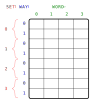
\includegraphics[width=.5\textwidth]{cache_logic_structure}
	\caption{Cache logic structure.}
	\label{fig:cache_logic_structure}
\end{figure}

Whenever a word $w$ is requested there are two possibilities:
\begin{itemize}
	\item \emph{Hit}: $w$ is present in the cache: the request can be
		immediately fulfilled.
	\item \emph{Miss}: $w$ is not present in the cache: it is necessary to
		retrieve it from lower level memory before fulfilling the request.
\end{itemize}
During the data retrieving a cache line is filled with a block of contiguous
words loaded from the lower level memory, trying to exploit spatial locality of
future accesses, while mapping policies and replacement policies determine which
cache line to overwrite, trying to exploit temporal locality.

If the cache memory is writable, data consistency is ensured by a consistency policy.
\subsection{Policies}
\subsubsection{Mapping policy}
The mapping policy is in charge of statically associating a lower level memory
line to a cache set.

The \emph{set associative} policy is the most common mapping policy: given a
cache memory with $s$ sets of $w$ words, the word address (referred to the lower
level memory) bits are split into three parts (as shown in
Figure~\ref{fig:address_partitioning}):
\begin{enumerate}
	\item $\log_2(w)$: offset of the word in the line.
	\item $\log_2(s)$: set.
	\item remaining MSBs: tag identifying the specific line.
\end{enumerate}

\begin{figure}
	\centering
	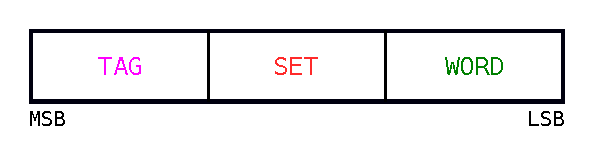
\includegraphics[width=.5\textwidth]{address_partitioning}
	\caption{Set associative policy address bits meaning.}
	\label{fig:address_partitioning}
\end{figure}

Special cases of this policy are:
\begin{itemize}
	\item \emph{Direct mapped} policy: each set is composed of a single line:
		the set bits identify a specific cache line, therefore there is
		no need for a replacement policy.
	\item \emph{Fully associative} policy: there is only a single set,
		therefore the line is fully determined by the replacement policy.
\end{itemize}

\subsubsection{Replacement policy}
The replacement policy is in charge of dynamically associating a lower level
memory line to a cache line of a set.

Multiple solutions of this problem have been developed, trying to maximize
the temporal locality exploitation.
Among the most commonly used solutions there are:
\begin{itemize}
	\item \emph{First-In First-Out}: the line to be replaced is the first
		one that has been inserted to the cache.
	\item \emph{Least recently used}: the line to be replaced is the one
		that has least recently been accessed.
\end{itemize}

\subsubsection{Consistency policy}
The consistency policy is in charge of ensuring data consistency between memories
belonging to different hierarchy levels.

The most common solutions to this problem are:
\begin{itemize}
	\item \emph{Write-back}: write accesses are performed to the highest
		level memory and lower level memories are updated when the cache
		line is replaced only.
	\item \emph{Write-through}: each write access is propagated along the
		whole hierarchy.
\end{itemize}

\section{FPGAs}
Field Programmable Gate Arrays are integrated circuits able to implement special
purpose circuits described in HDL, thanks to their programmable logic blocks and
interconnections.
\subsection{Memory system}
An FPGA memory system is typically made up of:
\begin{itemize}
	\item registers: the fastest but most expensive memories, therefore
		there are only a few.
	\item block RAMs: on chip RAMs accessible through simple and fast
		interface.
	\item external DRAM: off chip RAMs through complex and slow interface
		(e.g. AXI).
\end{itemize}

\section{High-Level Synthesis}
The High-Level Synthesis (HLS) is an Electronic Design Automation technique
aimed at translating an algorithm description in an high-level software
programming language (such as C and C++) into an Hardware Description Language
(HDL) description.

HLS allows to design more complex systems in less time, compared to HDL design,
moreover makes the hardware and software co-design much easier, at the cost of
less expressiveness.

\subsection{Workflow}
The typical HLS workflow consists of:
\begin{enumerate}
	\item software implementation: the top level entity is a C function:
		the function arguments are the entity ports and the functionality
		is implemented in SW; in order to guarantee synthesizability
		some constraints should be respected (e.g. no dynamic memory
		allocation).
	\item software verification: the testbench can be developed as a simple
		main function which calls the top level entity function,
		therefore the functionality is verified like any SW:
		it is possible to exploit traditional tools (e.g. debuggers,
		print statements...).
	\item hardware synthesis: the synthesizer generates an RTL description
		of the top level entity. It is possible to generate different
		architectures by setting up some parameters through dedicated
		directives.
	\item hardware verification: the RTL description is simulated, to make
		sure that SW and HW outputs match.
\end{enumerate}

\subsection{Optimization techniques}
Typical optimization techniques used by HLS for improving performance include:
\begin{itemize}
	\item pipelining: loops and functions logic can be pipelined so that
		successive iterations/calls can start while previous ones are
		still running. The introduced parallelism allows to increase
		the throughput at a limited additional area cost (only pipeline
		registers and an FSM are required).
	\item dataflow: different functions composing the design are called in
		a pipelined fashion (similarly to pipelining, but at task level,
		instead of instruction level).
	\item loop unrolling: the loop logic is instantiated multiple times,
		to execute multiple loop iterations in parallel, reducing latency
		and improving throughput.
	\item memory optimizations
		\begin{itemize}
			\item bursting: multiple memory accesses are aggregated
				to reduce overall latency and improving throughput.
			\item interface widening: multiple data elements are
				packed into a single bigger word, to perform
				multiple accesses at the same time.
		\end{itemize}
\end{itemize}

\iffalse
\section{\texttt{C++14}}
\subsection{Templates}
\texttt{C++} templates are a special kind of classes and functions arguments
which can be of any type (even type specifiers) and are evaluated at compile
time.
This mechanism allows to write generic code: the actual values are automatically
replaced before compilation, similarly to ``\texttt{\#define}'' preprocessor
directives.

\bigskip
The \emph{SFINAE} (Substitution Failure Is Not An Error) technique allows
to make the compiler ignore parts of code when the template substitution is
invalid, instead of throwing an error.
This technique is particularly effective when used together with the
\texttt{std::enable\_if} construct which conditionally returns an invalid type.

\subsection{Assertions}
\fi

\section{Previous work}\label{sec:liang}
Liang Ma et al. proposed an inlined cache implementation \cite{liang} in the form
of a set of \texttt{C++} classes: each of them implements an access type (read
only, write only and read write) and a mapping policy (direct mapped and set
associative).

Each cache is associated with a specific array stored to off-chip DRAM and
stores its data to on-chip BRAMs and registers. Since the cache is dedicated to
a specific array and the accesses to a single array are usually regular it is in
general easy to setup the different parameters to get high hit ratios.

The \texttt{operator[]} has been overloaded such that the cache can be used in
the same way of arrays, allowing to reduce the coding efforts when integrating
the cache in an existing algorithm.

During the synthesis the cache is inlined in the user algorithm: this may
clutter the logic and limit the maximum achievable performance.

\chapter{Basic architecture}
The fundamental idea behind the basic architecture
(Figure~\ref{fig:basic_arch}) is to keep application and cache logic into
separate processes, in order to simplify synthesis process: the cache should
always perform in the same manner, independently from the kernel in which it is
used, since it is separate from it, and the kernel algorithm may get better
performance, since it would only contain FIFO accesses instead of the entire
cache logic.

\bigskip
From the functional point of view, when application needs to access memory:
\begin{enumerate}
	\item application writes the request to the request FIFO.
	\item cache reads the request FIFO and checks if it causes a miss
	\item in case of miss, cache issues a request to the AXI interface to
		prepare its own memory (mapped to BRAM) for fulfilling the
		requested access.
	\item cache performs the access to BRAM and writes the outcome to the
		response FIFO (in case of a read request).
\end{enumerate}

\begin{figure}
	\centering
	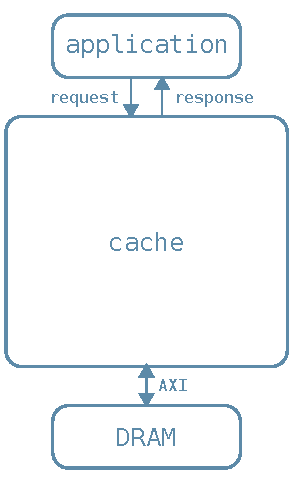
\includegraphics[width=.3\textwidth]{basic_arch}
	\caption{Single-process cache architecture.}
	\label{fig:basic_arch}
\end{figure}

\section{Single-process basic architecture}
This first proposed architecture is composed of a single pipelined process
which performs all the cache functionalities.

In case of Read-Only memory accesses this process can be pipelined with an
Initiation Interval of 1, while write accesses generate some dependencies on the
AXI interface which cause the process II to increase, dropping cache
performance.

\subsection{Implementation}
The single-process basic architecture has been implemented in the form of a
\texttt{C++14} class, compatible with \emph{Vitis HLS 2021.1}.

It is compliant with the set associative mapping policy and the write-back
consistency policy.
Template parameters allow to select word type, number of words per line, number
of sets and ways (therefore it is possible to obtain a fully associative policy
by setting the number of sets to 1 or a direct mapped policy by setting the
number of ways to 1).
It is also possible to select the replacement policy between Least Recently Used
and Last-In First-Out.

\subsubsection{Multi-process modeling}
HLS is intended for synthesizing sequential software code, therefore it has
been necessary to develop a novel technique for modeling multi-process designs.

A process is modeled as an infinite loop and their parallelism is modeled
differenlty depending on the compilation target:
\begin{itemize}
	\item \emph{SW simulation}: each process is mapped to an
		\texttt{std::thread}.
	\item \emph{HW synthesis}: each process is a dataflow function, in a
		dataflow region with the \texttt{disable\_start\_propagation}
		option disabled (which allow each function to run in parallel,
		without waiting for the completion of previous ones).
\end{itemize}
The distinction between simulation and synthesis code can be performed through
the ``\texttt{\#ifdef \_\_SYNTHESIS\_\_}'' preprocessor directive.

Different processes can communicate by means of FIFOs (\texttt{hls::stream}
provided by Vitis HLS), which allow unidirectional point-to-point communication
between two processes. It is possible to insert multiple FIFOs between each
process, in both directions, therefore allowing to setup duplex communication.

Since \texttt{hls::stream} provides blocking operations, these FIFOs can be also
used for synchronization purposes.

\subsubsection{RAW dependencies}
The cache process II is limited by the Read-After-Write dependencies on the
cache lines, therefore the RAW cache has been developed: it is a single-line
cache which provides the functions:
\begin{itemize}
	\item \texttt{get\_line}: in case of hit, read the RAW cache line;
		in case of miss, read the cache line.
	\item \texttt{set\_line}: write both the RAW cache line and the cache
		line.
\end{itemize}

The cache process always accesses cache memory through the RAW cache and it
calls the \texttt{set\_line} function once per iteration at most: if a cache
line has been written it is impossible that it is read in the next iteration,
since the RAW cache would hit and return its line. This allows to falsify the
RAW dependency with distance of 1 on the cache memory, making it possible to
schedule the cache process with an II of 1.

\section{Multi-processes basic architecture}
In this architecture, the cache have been split into two processes
(Figure~\ref{fig:basic_arch_inner}):
\begin{itemize}
	\item core: manage communication with application and keep cache data
		structures up to date.
	\item memory interface: deal with the AXI interface.
\end{itemize}

This solution allows to pipeline the \emph{core} process with an II of one, even
in case of write accesses, since the AXI interfacing resides in the separate
\emph{memory interface} process.

The latency of the response to an hitting request depends on the \emph{core}
process only, therefore with this solution desired performance is achieved in
case of writable caches too.

\begin{figure}
	\centering
	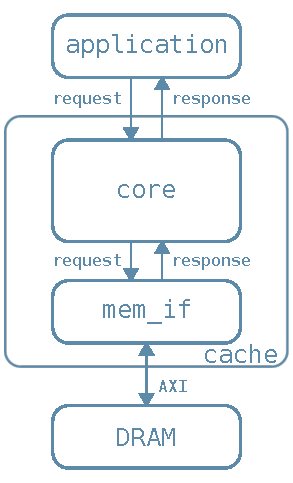
\includegraphics[width=.3\textwidth]{basic_arch_inner}
	\caption{Multi-processes cache architecture.}
	\label{fig:basic_arch_inner}
\end{figure}

\chapter{Optimized architectures}
\section{L1 cache}
Each FIFO access costs one clock cycle, which has to be paid for each memory
access. 
To improve performance each read request to the cache does not return a single
data element, but a whole cache line. This allows to insert a Level 1 cache
above the underlying cache, directly inlined in the user logic, similarly to
the cache described in Section~\ref{sec:liang}.

Since it is important not to clutter the user logic, the L1 cache is kept as
simple as possible: it complies with the direct mapped mapping policy and the
write-through consistency policy.

The read accesses only can benefit from the L1 cache insertion, due to the
write-through consistency policy: read accesses are usually more frequent than
write accesses, therefore the optimization efforts has been focused on them.

\begin{figure}
	\centering
	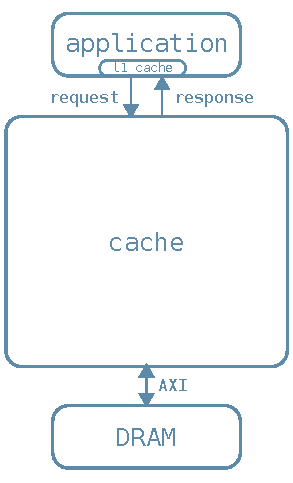
\includegraphics[width=.3\textwidth]{l1_arch}
	\caption{Cache architecture optimized with the insertion of a L1 cache.}
	\label{fig:l1_arch}
\end{figure}

\section{Multiple ports}
The vast majority of algorithms access memory inside loops, which in HLS can be
optimized in two main ways: pipelining, which perfectly fits the single-port
cache architecture, and unrolling, with which the II would increase, since each
unrolled iteration should access the same FIFO at the same time.

To solve this problem a multi-port architecture is proposed: each port has
dedicated FIFOs and the cache process serves each request in order.
Each port has also a dedicated L1 cache, which can be used without any
coherency problem, since they follow the write-through consistency policy.


\chapter{Results}
\section{Matrix multiplication}
\section{Bitonic sorting}
\section{Lucas-Kanade}

\chapter{Conclusion}

\printbibliography

\end{document}

